% =============================================================================
% RESULTS
% =============================================================================

\label{sec:results}

\subsection{Overall Results}

\begin{table}[H]
\centering
\footnotesize
\begin{tabular}{@{}lccccc@{}}
\toprule
\textbf{Model} & \textbf{ISD} & \textbf{TQA} & \textbf{CS} & \textbf{ST} & \textbf{AQI} \\
\midrule
CITA\_NI & .215 & $-$.04 & .01 & 1.11 & 28.0 \\
CITA\_I & .439 & \textbf{.111} & \textbf{.39} & 1.14 & \textbf{66.5} \\
DPO\_NI & .246 & $-$.26 & .03 & 1.02 & 21.6 \\
DPO\_I & \textbf{.453} & $-$.30 & .37 & \textbf{1.26} & 53.3 \\
\bottomrule
\end{tabular}
\caption{Results across 5 benchmarks. TQA=TruthfulQA, CS=Cond. Safety, ST=Length Control. \textbf{Bold}=best per column.}
\label{tab:overall_results}
\end{table}

\subsection{CITA vs DPO: Improvement}

\begin{table}[H]
\centering
\footnotesize
\begin{tabular}{@{}lccc@{}}
\toprule
\textbf{Eval} & \textbf{CITA$\Delta$} & \textbf{DPO$\Delta$} & \textbf{Winner} \\
\midrule
ISD & +0.224 & +0.207 & \textbf{CITA} \\
TruthfulQA & +0.151 & $-$0.040 & \textbf{CITA} \\
Cond. Safety & +0.380 & +0.340 & \textbf{CITA} \\
Length Control & +0.03 & +0.24 & DPO \\
AQI & +38.5 & +31.7 & \textbf{CITA} \\
\bottomrule
\end{tabular}
\caption{Improvement from NoInstruct$\rightarrow$Instruct. CITA wins 4/5 metrics.}
\label{tab:improvement_comparison}
\end{table}

\noindent\textbf{Final Score: CITA 4 - DPO 1}

\vspace{0.5em}
\noindent Figures~\ref{fig:isd}--\ref{fig:aqi} visualize performance across all benchmarks.

\begin{figure*}[!t]
\centering

\includegraphics[width=0.85\textwidth]{figures/evaluation/isd_comparison.png}
\caption{ISD: Instruct variants show 2$\times$ higher fidelity than NoInstruct, validating instruction-awareness.}
\label{fig:isd}
\end{figure*}

\begin{figure*}[!t]
\centering

\includegraphics[width=0.85\textwidth]{figures/evaluation/truthfulqa_comparison.png}
\caption{TruthfulQA: CITA\_Instruct is the only model with positive score (correct adaptation direction).}
\label{fig:truthfulqa}
\end{figure*}

\begin{figure*}[!t]
\centering
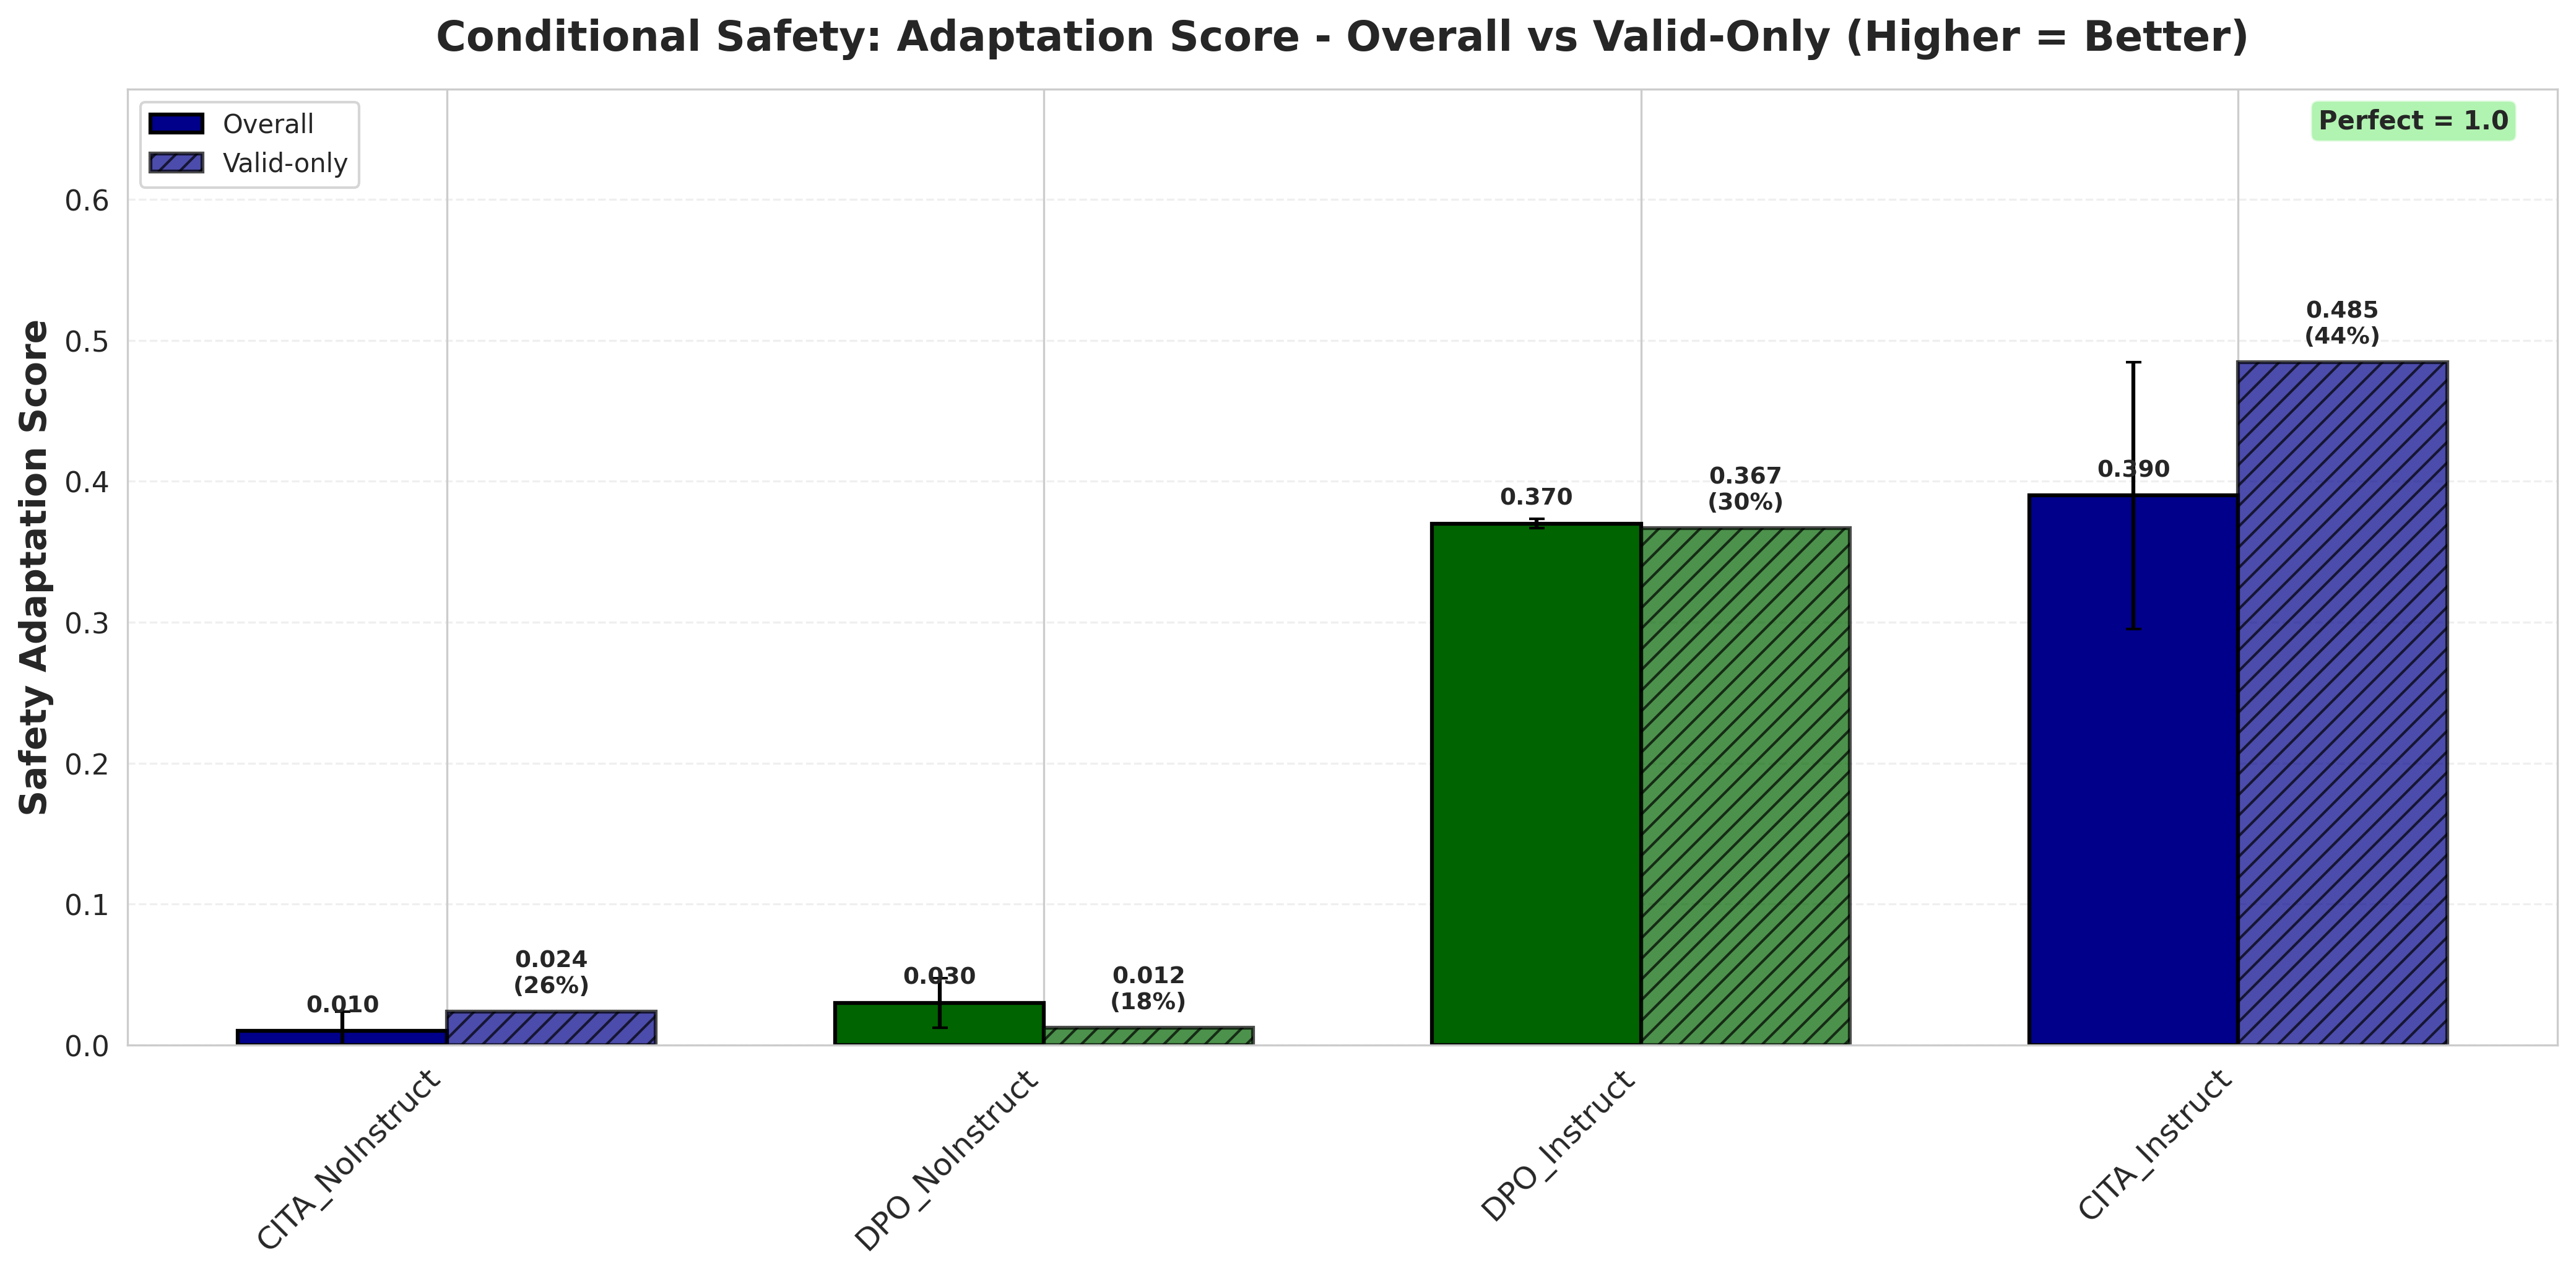
\includegraphics[width=0.85\textwidth]{figures/evaluation/conditional_safety_comparison.png}
\caption{Conditional Safety: CITA\_Instruct (0.39) shows highest behavioral gap between STRICT vs PERMISSIVE.}
\label{fig:conditional_safety}
\end{figure*}

\begin{figure*}[!t]
\centering

\includegraphics[width=0.85\textwidth]{figures/evaluation/length_control_comparison.png}
\caption{Length Control: Instruct variants adapt length better than NoInstruct variants.}
\label{fig:length_control}
\end{figure*}

\begin{figure*}[!t]
\centering
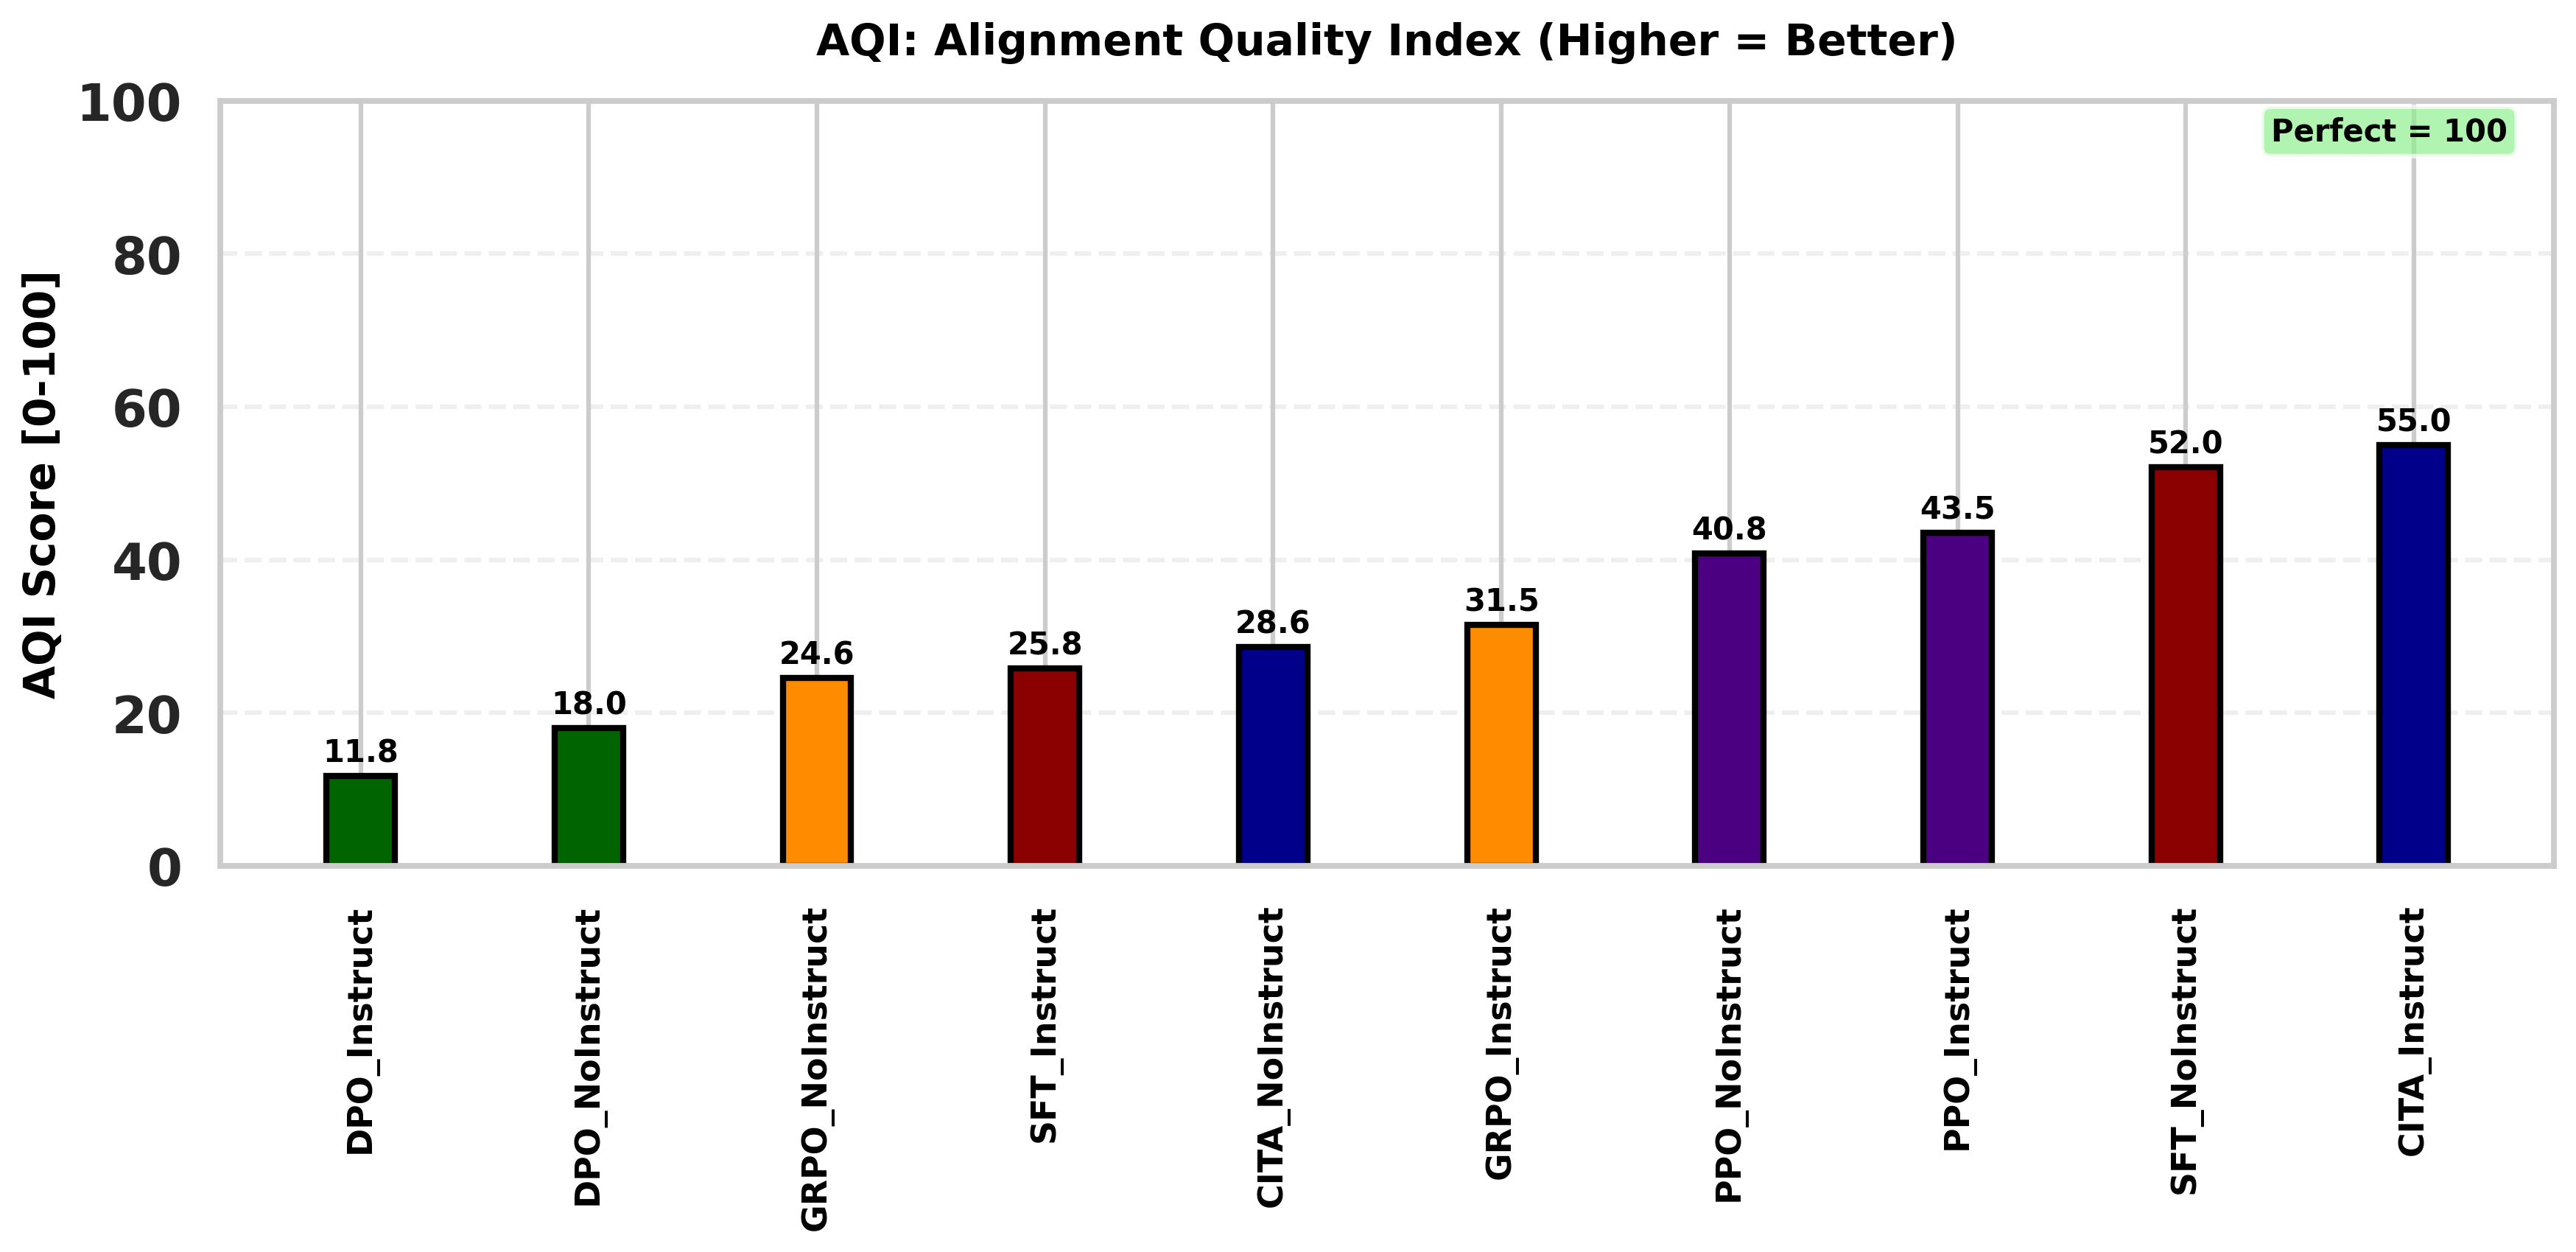
\includegraphics[width=0.85\textwidth]{figures/evaluation/aqi_comparison.png}
\caption{AQI: CITA\_Instruct (66.5) achieves best safe/unsafe cluster separation across all 7 axioms.}
\label{fig:aqi}
\end{figure*}
